% "{'classe':('PSI'),'chapitre':'cin_va','type':('td'),'titre':'Centrifugeuse humaine', 'source':'','comp':(''),'corrige':True}"

\chapter*{Application \arabic{cptApplication} \\ 
Centrifugeuse humaine -- \ifprof Corrigé \else Sujet \fi}
\addcontentsline{toc}{section}{Application \arabic{cptApplication} : Centrifugeuse humaine -- \ifprof Corrigé \else Sujet \fi}

\iflivret \stepcounter{cptApplication} \else
\ifprof  \stepcounter{cptApplication} \else \fi
\fi

\setcounter{question}{0}
%\marginnote{Ressources de l'équipe pédagogique La Martinière Monplaisir.}
\marginnote[1cm]{
%\UPSTIcompetence[2]{B2-14}
%\UPSTIcompetence[2]{C1-05}
%\UPSTIcompetence[2]{C2-07}
}






Afin d'analyser les effets de l'accélération sur le corps humaine, le CNRS / MEDES a développé une centrifugeuse humaine. On donne ci-dessous la modélisation cinématique de la centrifugeuse.

\begin{center}
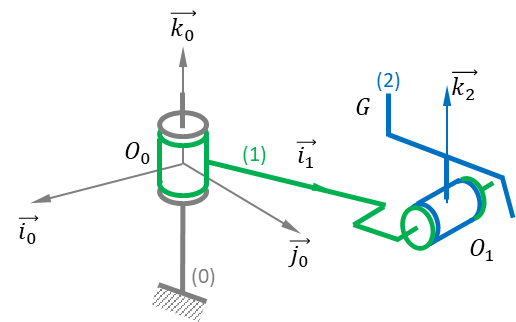
\includegraphics[height=4cm]{centrifugeuse_2}

%\textit{Modélisation cinématique} 
\end{center}


Le paramétrage de la centrifugeuse est donnée ci dessous : 



\begin{center}
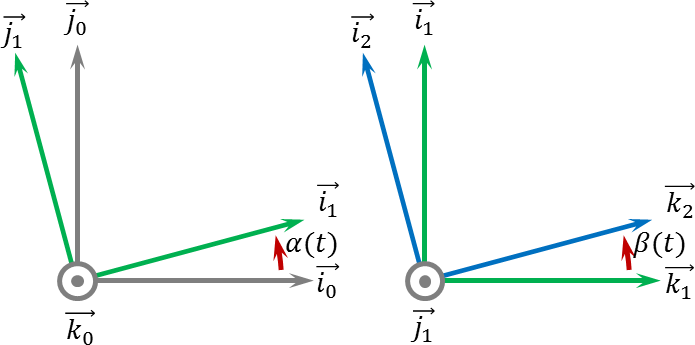
\includegraphics[height=3cm]{centrifugeuse_3}
\end{center}

Les paramètres constants du système sont les suivants : 
\begin{itemize}%[$\bullet$]
\item $\vect{O_0O_1} = a \vect{i_1}$;
\item $\vect{O_1G} = b \vect{i_2} + c \vect{k_2}$.
\end{itemize}


\subsection*{Trajectographie}

\question{Donner la trajectoire du point $G$ dans le repère $\mathcal{R}_0$.}
\ifprof
\begin{corrige}
La trajectoire du point $G$ dans le repère $\mathcal{R}_0$  est donnée par le vecteur :
$$
\vect{O_0 G}(t)  = \vect{O_0O_1} + \vect{O_1G}
= a \vect{i_1} +  b \vect{i_2} + c \vect{k_2}
$$

Il faut alors projeter les vecteurs dans $\mathcal{R}_0$ : 
\begin{eqnarray*}
\vect{O_0 G}(t) &=& a \left(\cos\alpha(t) \vect{i_0} + \sin\alpha(t) \vect{j_0} \right) 
+ b \left(\cos\beta(t) \vect{i_1} - \sin\beta(t) \vect{k_1} \right) 
+ c\left(\cos\beta(t) \vect{k_1} + \sin\beta(t)\vect{i_1}\right)\\
&=& a \left(\cos\alpha(t) \vect{i_0} + \sin\alpha(t) \vect{j_0} \right) 
+ b \left(\cos\beta(t) \left(\cos\alpha(t) \vect{i_0} + \sin\alpha(t) \vect{j_0} \right) - \sin\beta(t) \vect{k_0} \right) \\
&& + c\left(\cos\beta(t) \vect{k_0} + \sin\beta(t)  \left(\cos\alpha(t) \vect{i_0} + \sin\alpha(t) \vect{j_0} \right) \right)\\
&=& \left[ \begin{array}{c} 
a \cos\alpha(t) + b \cos\beta(t) \cos\alpha(t) +c \sin\beta(t)\cos\alpha(t)\\
a \sin\alpha(t) + b \cos\beta(t) \sin\alpha(t) +c \sin\beta(t)\sin\alpha(t) \\
- b\sin\beta(t) + c\cos\beta(t)
\end{array}\right]_{\mathcal{R}_0}
\end{eqnarray*}

On a ainsi l'équation paramétrique de la position du point $G$.

\end{corrige}
\else \fi


\subsection*{Cinématique}
%
%\question{Donner la trajectoire du point $G$ dans le repère $\mathcal{R}_0$.}
%
%\question{Calculer $\vectv{O_0}{S_1}{S_0}$ et $\vectv{O_1}{S_2}{S_1}$.}

\question{Calculer $\vectv{G}{S_2}{S_0}$.}



%
%\question{Calculer $\vectv{G}{S_2}{S_0}$.}

\subsection*{Accélération}

\question{Calculer $\vectg{G}{S_2}{S_0}$.}


\ifprof
\begin{corrige}


\textbf{Méthode 1 -- PAS RECOMMANDE }
Par définition, 
$$
\vectv{O_1}{S_1}{S_0} 
= \left[\dfrac{\text{d}\vect{O_0O_1}(t)}{\text{d}t}\right]_{\mathcal{R}_0}
= \left[\dfrac{\text{d} \left(a \vect{i_1}\right) }{\text{d}t}\right]_{\mathcal{R}_0}
= a \left[\dfrac{\text{d}  \vect{i_1} }{\text{d}t}\right]_{\mathcal{R}_0}
$$

On a :
\begin{eqnarray*}
\left[\dfrac{\text{d}  \vect{i_1} }{\text{d}t}\right]_{\mathcal{R}_0}
&=&\left[\dfrac{\text{d} \left(\cos\alpha(t)\vect{i_0}+\sin\alpha(t)\vect{j_0} \right)}{\text{d}t}\right]_{\mathcal{R}_0}
=\left[\dfrac{\text{d}  \cos\alpha(t)\vect{i_0}}{\text{d}t}\right]_{\mathcal{R}_0}
+\left[\dfrac{\text{d}  \sin\alpha(t)\vect{j_0} }{\text{d}t}\right]_{\mathcal{R}_0}\\
& = & 
\dfrac{\text{d} \cos\alpha(t)}{\text{d}t} \vect{i_0}  
+\cos\alpha(t)\underbrace{\left[\dfrac{\text{d}  \vect{i_0}}{\text{d}t}\right]_{\mathcal{R}_0}}_{\vect{0}}
+\dfrac{\text{d} \sin\alpha(t)}{\text{d}t} \vect{i_0}  
+\sin(t)\underbrace{\left[\dfrac{\text{d}  \vect{j_0}}{\text{d}t}\right]_{\mathcal{R}_0}}_{\vect{0}}\\
& = & -\dot{\alpha}(t)\sin\alpha(t) \vect{i_0}   + \dot{\alpha}(t)\cos\alpha(t) \vect{j_0}  = 
\dot{\alpha}(t)\vect{j_1}
\end{eqnarray*}

Ainsi,
$$
\vectv{O_1}{S_1}{S_0} 
= \left[\begin{array}{c} 
-a\dot{\alpha}(t)\sin\alpha(t) \\
a \dot{\alpha}(t)\cos\alpha(t) \\
0 \end{array}\right]_{\mathcal{R}_0}
=\left[\begin{array}{c} 0 \\ a\dot{\alpha}(t) \\ 0\end{array}\right]_{\mathcal{R}_1}
$$

Dans les deux cas, $\vect{O_0O_1}(t)$ est dérivé par rapport $\mathcal{R}_0$ mais il s'exprime différemment dans $\mathcal{R}_0$ et $\mathcal{R}_1$ :
\begin{itemize}
\item $\vectv{O_1}{S_1}{S_0} = -a\dot{\alpha}(t)\sin\alpha(t) \vect{i_0}   + a\dot{\alpha}(t) \cos\alpha(t) \vect{j_0}$ : ici la base de \textbf{projection} et de \textbf{dérivation} est la base $\mathcal{B}_0$;
\item $\vectv{O_1}{S_1}{S_0} = a\dot{\alpha}(t)\vect{j_1}$ : ici la base de dérivation est la base $\mathcal{B}_0$ et la base de projection est $\mathcal{B}_1$.
\end{itemize}


\textbf{Méthode 2 -- Utilisation de la dérivation vectorielle.}

Calcul de $\vectv{O_1}{S_1}{S_0}$.

On rappelle que :
$$
\vectv{O_1}{S_1}{S_0} 
= a \left[\dfrac{\text{d}  \vect{i_1} }{\text{d}t}\right]_{\mathcal{R}_0}
$$

Le calcul de $\left[\dfrac{\text{d}  \vect{i_1} }{\text{d}t}\right]_{\mathcal{R}_0}$ peut donc être réalisé ainsi : 
$$ 
\left[\dfrac{\text{d}  \vect{i_1} }{\text{d}t}\right]_{\mathcal{R}_0} = 
\underbrace{\left[\dfrac{\text{d}  \vect{i_1} }{\text{d}t}\right]_{\mathcal{R}_1}}_{\vect{0}} + \vecto{S_1}{S_0}\wedge \vect{i_1}
=\dot{\alpha}\vect{k_0}  \wedge \vect{i_1}
=\dot{\alpha} \vect{j_1}
$$

Ainsi 
$$
\vectv{O_1}{S_1}{S_0} 
= a \dot{\alpha} \vect{j_1}
$$

\textbf{Méthode 3 -- }
Calcul de $\vectv{O_1}{S_1}{S_0}$.

$S_1$ et $S_0$ sont en liaison pivot de centre $O_0$, on a donc :  $\vectv{O_0}{S_1}{S_0}=\vect{0}$.

En conséquence, 
$$
\vectv{O_1}{S_1}{S_0} = \vectv{O_0}{S_1}{S_0} + \vect{O_1O_0}\wedge   \vecto{S_1}{S_0} = \vect{0} - a \vect{i_1} \wedge \left( \dot{\alpha}\vect{k_0} \right)
=a \dot{\alpha}\vect{j_1}
$$

\end{corrige}\else \fi

%
%\subparagraph{}
%\textit{Calculer $\vecto{S_1}{S_0}$, $\vecto{S_2}{S_1}$ et $\vecto{S_2}{S_0}$.}
%
%
%
%\subparagraph{}
%\textit{Calculer $\vectv{G}{S_2}{S_0}$.}
\ifprof
\begin{corrige}

Calcul de $\vectv{G}{S_2}{S_0}$.
%On a :
%$$\vecto{S_2}{S_0}=\vecto{S_2}{S_1}+\vecto{S_1}{S_0} = \dot{\alpha}\vect{k_0} + \dot{\beta}\vect{j_1}  $$

%Par ailleurs, 
On a : 
$$\vectv{G}{S_2}{S_0} = \vectv{G}{S_2}{S_1} + \vectv{G}{S_1}{S_0} $$
Calculons $\vectv{G}{S_1}{S_0}$ :
$$
\vectv{G}{S_1}{S_0} 
= \vectv{O_1}{S_1}{S_0} + \vect{GO_1}\wedge\vecto{S_1}{S_0}
= a\dot{\alpha}\vect{j_1} - \left(b\vect{i_2} + c\vect{k_2}\right) \wedge\left( \dot{\alpha} \vect{k_0}\right)
$$
$$
\vectv{G}{S_1}{S_0} 
= a\dot{\alpha}\vect{j_1}  + b\dot{\alpha} \sin(\beta+\pi/2) \vect{j_1} + c \dot{\alpha}\sin\beta\vect{j_1}
= \dot{\alpha} \left(a+b \cos\beta + c \sin\beta\right) \vect{j_1} 
$$

Par ailleurs calculons $\vectv{G}{S_2}{S_1}$ :
$$\vectv{G}{S_2}{S_1} = \vectv{O_1}{S_2}{S_1} + \vect{GO_1}\wedge \vecto{S_2}{S_1}
=-\left(b\vect{i_2}+c\vect{k_2}\right) \wedge \left(\dot{\beta}\vect{j_1}\right)
=-\dot{\beta}\left(b\vect{k_2}-c\vect{i_2} \right)
$$

Au final, 
$$\vectv{G}{S_2}{S_0} = \dot{\alpha} \left(a+b \cos\beta + c \sin\beta\right) \vect{j_1} 
-\dot{\beta}\left(b\vect{k_2}-c\vect{i_2} \right)
$$

Il est aussi possible de calculer $\vectv{G}{S_2}{S_0}$ ainsi : 
$$\vectv{G}{S_2}{S_0} = \left[\dfrac{\text{d} \vect{O_0G}}{\text{d}t}\right]_{\mathcal{R}_0}$$ 

\end{corrige}\else \fi

